In this section, we present and analyze the results obtained from the experiments conducted on the methods introduced in the previous chapters. For each macro category, we implemented two algorithmic approaches. Our analysis is divided into two phases: first, we fine-tune the main parameters (when applicable), and then we compare the best-performing configurations within each category.

\section{Methodology}

Each group of algorithms will be analyzed independently following a consistent methodology. Three main parameters are considered in all experiments:
\begin{itemize}
    \item \textbf{Number of nodes:} This varies depending on the nature of the method (e.g., fewer nodes for exact methods, more for heuristics and metaheuristics).
    \item \textbf{Time limit:} Fixed for each experiment to ensure comparability across algorithms.
    \item \textbf{Number of runs:} Each configuration is tested on 20 different randomly generated instances to guarantee statistical significance.
\end{itemize}

To enable a rigorous comparison, we rely on \textbf{Performance Profiles}, a graphical tool that allows us to assess and visualize the comparative efficiency of different algorithms across a suite of problem instances.

\subsection{Instance Generation}

The TSP instances used in our experiments are generated randomly. Each instance consists of a set of points placed on a 2D grid $[0, 10\,000] \times [0, 10\,000]$, with coordinates sampled from an i.i.d. uniform distribution. The cost matrix for each instance is computed using the Euclidean distance between points, optionally rounded according to the ATT formula from TSPLIB.

\subsection{Experimental Setup}

All experiments were conducted on a machine equipped with an Intel Core i7-10510U processor and 16 GB of RAM. The exact methods were solved using \textbf{IBM ILOG CPLEX 22.1.2}, interfaced via its C API. Heuristic and metaheuristic algorithms were developed in C for performance, while Python was used to manage experiment automation and result visualization.

\subsection{Performance Profiles}

To compare the performance of different algorithms across a common set of instances, we used performance profiles. These were generated with a Python script developed by Domenico Salvagnin. The script processes a CSV table containing the results of each algorithm on each instance, and compares the performance of each algorithm to the best obtained on the same instance.
This approach enables us to build plots that show, for each algorithm, how often it performs within a certain range of the best result, offering a clear visual summary of relative performance. For heuristics and metaheuristics, the comparison is based on the cost of the best solution found; for exact methods, on the time required to find the optimal solution.

For each class of methods, the following parameters were used in the experiments:
\begin{itemize}
    \item \textbf{Heuristics:} 1000-node instances, time limit of 120 seconds.
    \item \textbf{Metaheuristics:} 1000-node instances, time limit of 120 seconds.
    \item \textbf{Exact methods:} 200-node instances, time limit of 120 seconds.
    
    
\end{itemize}

Each test was repeated over 20 instances, initialized with different random seeds. All results are reported in the form of performance profiles to ensure clarity and comparability.

\section{Parameters tuning}

\subsection{Tabu Search}
\label{ssec:tabu-tuning}
As discussed in Section~\ref{sec:tabu}, Tabu Search relies on a short-term memory of forbidden moves, whose size is governed by the base tenure \(T\).  In many works one selects a single ratio \(\alpha\) and sets \(T=\frac{N_{\mathrm{nodes}}}{\alpha}\), but this hides the fact that the method can be tuned more flexibly by independently controlling the dynamic bounds \(T_{\min}\) and \(T_{\max}\).

In our implementation we therefore allow the user to specify all parameters directly, allowing also for setting the cutoff for forced diversification, \(N_{\mathrm{ni}}\). Conceptually, however, it is still suggested to leverage the ratio \(\alpha\) to derive the base tenure \(T\).

Table~\ref{tab:tabu-configs} reports the eight configurations where we tried to span as many different search behaviors as possible.

\begin{table}[H]
  \centering
  \caption{Tabu search configurations}
  \label{tab:tabu-configs}
  \resizebox{\textwidth}{!}{%
  \begin{tabular}{|c|c|c|c|l|}
    \hline
    \textbf{$T$} & \textbf{$T_{\min}$} & \textbf{$T_{\max}$} & \textbf{$N_{\mathrm{ni}}$} & \textbf{Description} \\ 
    \hline
    227 & 10 & 227 & 500 & Good balance, but no expansion beyond the initial tenure. \\
    250 & 10  & 375  & 500  & Moderate diversification via expanded max tenure. \\ 
    208 & 5   & 416  & 1000 & Broad tenure span allows prolonged exploration before reset. \\ 
    278 & 20  & 278  & 250  & Fixed high tenure intensifies local moves with quick shake-up. \\ 
    167 & 10  & 167  & 500  & Small tenure forces rapid neighborhood changes. \\ 
    333 & 10  & 500  & 500  & Max tenure scaled to problem size supports deeper history. \\ 
    100 & 5   & 500  & 200  & Very short base tenure and low cutoff for intense shaking. \\ 
    400 & 50  & 400  & 2000 & Large tenure and high cutoff delay diversification for global search. \\ 
    \hline
  \end{tabular}%
  }
\end{table}

Results highlight that configurations with a large base tenure and a wide dynamic span tend to converge more quickly to high-quality incumbents. In particular:
\begin{itemize}
  \item \emph{High base tenure}: retaining a long short-term memory before forcing diversification produces the best overall performance, by exploiting promising regions.
  \item \emph{Wide dynamic window}: allowing the tabu tenure to expand and contract over a large interval helps escape local optima when progress stalls.
  \item \emph{Medium settings}: a moderate base tenure with a moderately sized dynamic range provides a reasonable trade-off between intensification and diversification, but does not match the extremes.
  \item \emph{Small or rigid tenure}: very short or fixed tabu lists lead to slower discovery of good solutions and a greater risk of stagnation.
\end{itemize}

\begin{figure}[H]
  \centering
  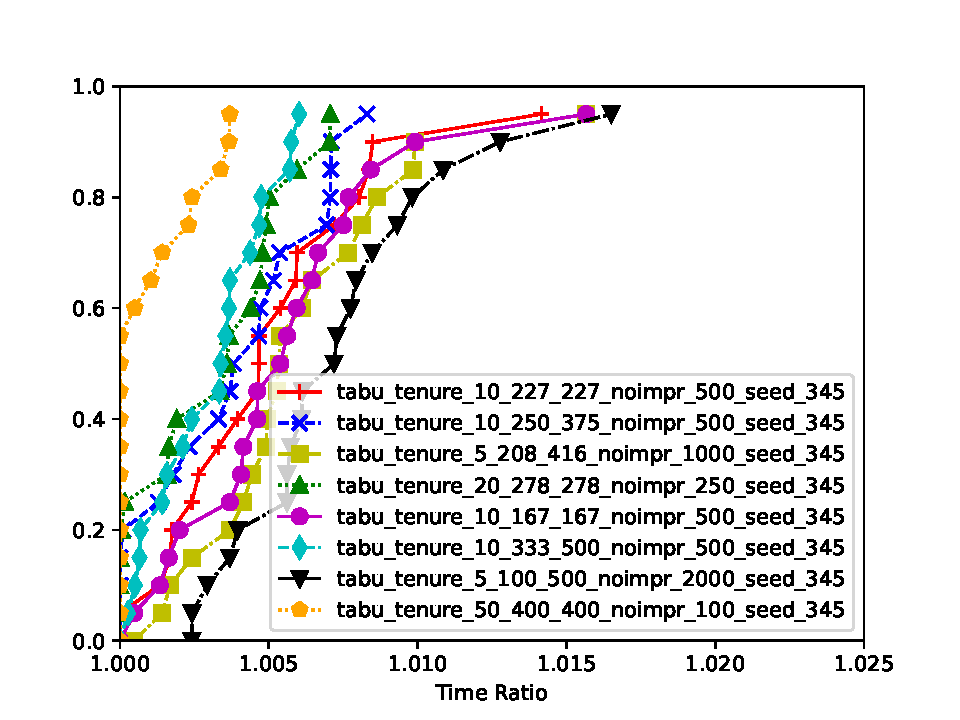
\includegraphics[width=0.8\textwidth]{tabu_profiles.pdf}
  \caption{Performance profiles for the Tabu Search configurations.}
  \label{fig:tabu-profiles}
\end{figure}

\subsection{Varable Neighborhood Search}
\label{ssec:vns-tuning}

To find the best configuration for the VNS algorithm, we focused on the parameters that control the number of 3-opt “kicks” applied per iteration. We let the user specify a fixed number of kicks \(J\) or an adaptive scheme that draws a number of kicks uniformly from a range \([k_{\min},k_{\max}]\), scaled by a learning rate \(\lambda\). Table~\ref{tab:vns-configs} summarizes the settings we evaluated:

\begin{table}[H]
  \centering
  \caption{VNS configurations}
  \label{tab:vns-configs}
  \resizebox{\textwidth}{!}{%
  \begin{tabular}{|c|c|c|c|c|l|}
    \hline
    \textbf{ID} & \(\boldsymbol{k_{\min}}\) & \(\boldsymbol{k_{\max}}\) & \(\boldsymbol{\lambda}\) & \(\boldsymbol{J}\) & \textbf{Description} \\ 
    \hline
    1 & 2   & 4   & 1.00 & -  & Balanced adaptive kicks. \\ 
    2 & 1   & 5   & 1.00 & -  & Wide range for broader exploration. \\ 
    3 & 2   & 6   & 1.00 & -  & Extended range for more diversification. \\ 
    4 & 1   & 10  & 1.00 & -  & Very wide span, high diversification. \\ 
    5 & 2   & 4   & 0.50 & -  & Conservative kicks (half learning rate). \\ 
    8 & 2   & 4   & 2.00 & -  & Aggressive kicks (double learning rate). \\ 
    6 & -   & -   & -    & 3  & Fixed few kicks per iteration. \\ 
    7 & -   & -   & -    & 10 & Fixed many kicks, conservative scale. \\ 
    \hline
  \end{tabular}%
  }
\end{table}

Results presented in Figure \ref{fig:vns-profiles} suggest that a fixed number of kicks per iterations is more effective than adaptive schemes. In particular, the more kicks are applied the better the results, with the with the configuration applying 10 kicks outperforming all others. Anyways, the adaptive schemes still perform reasonably well, especially when the range of kicks is wide enough to allow for sufficient exploration.

\begin{figure}[H]
  \centering
  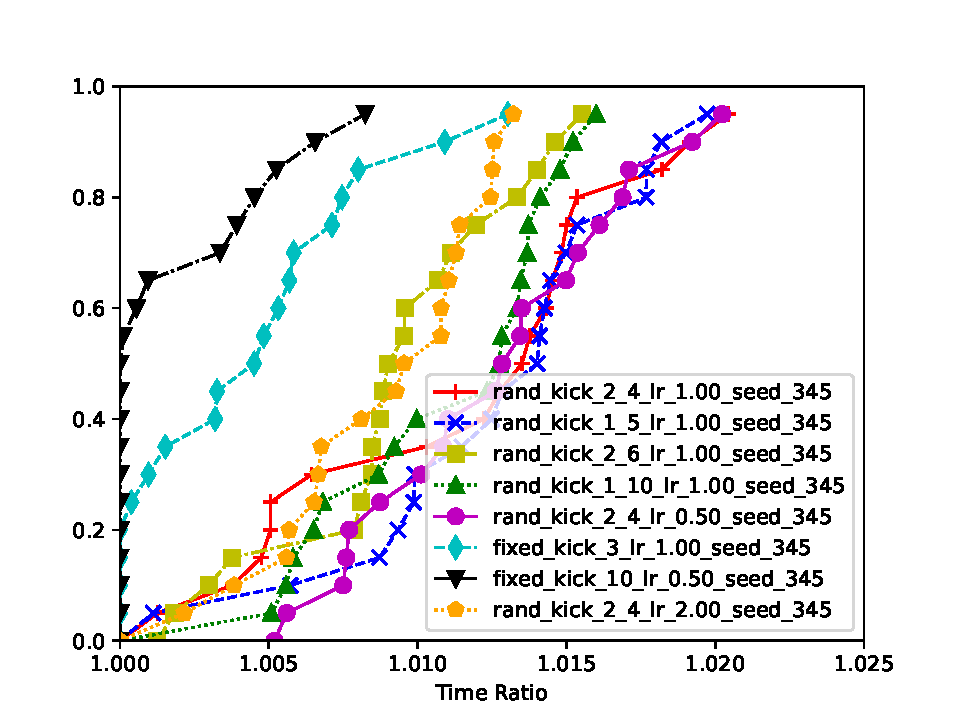
\includegraphics[width=0.8\textwidth]{vns_profiles.pdf}
  \caption{Performance profiles for the VNS configurations.}
  \label{fig:vns-profiles}
\end{figure}
